\section{Coherent Synchrotron Radiation}
\Gls{sr} is produced in synchrotron radiation facilites (like electron storage rings) by accelerating relativistic electrons.
Emission of \gls{sr} occurs, when electron beams are bend or deflected with dipole magnets or using an undulator\footnote{Undulators are used to make the electrons oscillate by generating a periodic magnetic field}. 

\autoref{fig:storageRing} shows the general scheme of an electron storage ring.
Electrons, or rather electron bunches, are generated with an electron gun and are accelerated to almost the speed of light by a \gls{linac}.
After being broad up to their nominal energy in a booster, the bunches are then injected into the storage ring.
In the ring, the path of the electron bunches is altered by bending magnets, guiding them on a circular trajectory.
Due to emission of \gls{sr} at each bend, the electrons lose energy, which has to be compensated for.
This is done by accelerating them with an electric field inside a \gls{rf} cavity.
Not shown in the drawing are the beamlines, which lead the \gls{sr} radiation, or rather chosen wavelength ranges, through an optical system to the respective user experiments. \cite{roussel2014} \cite{rota2018}

\begin{figure}[tbh]
 	\centering
 	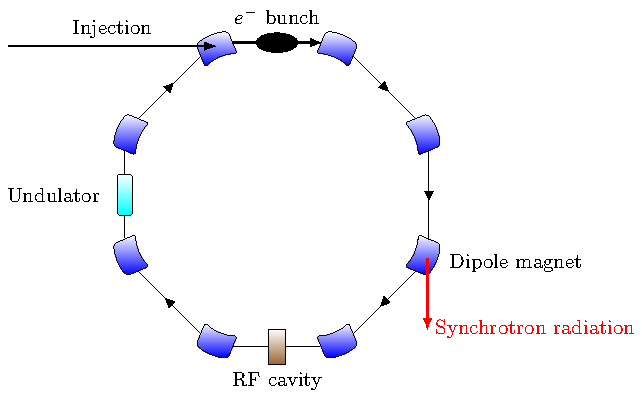
\includegraphics[width=0.7\textwidth]{chap/02-theory/img/synchrotron}
 	\caption{Basic scheme of an electron storage ring (redrawn from \cite{roussel2014})}
 	\label{fig:storageRing}
\end{figure}
%todo where's the booster?
 
 
The range of \gls{sr} reaches from hard X-rays down to the infrared region of the electromagnetic spectrum (see \autoref{fig:spectrum}). In contrast to other sources, it has properties like:
%todo which sources, convert list to text?
\begin{itemize}[noitemsep]
	\item high intensity 
	\item high collimation
	\item polarisation
	\item well-defined timing of pulses
\end{itemize}

Due to this properties, synchrotrons are used for microscopy, spectroscopy, and time-resolved experiments in such fields like condensed matter physics, biology, material science and many more.
%todo why are these imporant for the applications listed here. maybe pick one and explain it in more detail and/or an equation
\begin{figure}[H]
	\centering
	\includegraphics[width = 0.8\textwidth, height = 0.5\textwidth]{chap/02-theory/img/spectrum.tikz}
	\caption{Electromagnetic spectrum} %todo of what?
	\label{fig:spectrum}
\end{figure}
%todo legend -> 7 columns instead of one. or just label the ranges with 'big braces' directly
%todo replace with measured I(\lambda)/I_0 plot?

\subsection{Micro-Bunching Instabilities}
Increasing demands in current and future accelerators call for higher brilliance of the emitted radiation.
%todo define brilliance, flux, emittance
This is achieved by increased photon flux and reduction of the transverse emittance.
For longitudinal coherence, the electron bunches are shortened, which results in emission of \gls{csr} at frequencies up to the THz range.
%todo how does coherence relate to the terms mentioned earlier?

However, this introduces complex dynamics, as the electrons interact with their own radiation.
This manifests into the so called micro-bunching instability.
The formation of micro-structures (in the sub-millimeter to centimeter range) in the longitudinal density profile of the electron bunches. %todo AE or BE ('re' vs 're')?
Being on the one side a limitation to the stable operation of the overall system at high current density/short bunch length mode.
On the other side, these instabilities can be potential sources of brilliant THz radiation. %todo why
A thorough understanding of these dynamics is necessary to control the emission in this spectral domain which enables usage in experiments. \cite{rota2018,brosi}

\begin{figure}[tbh]
	\centering
	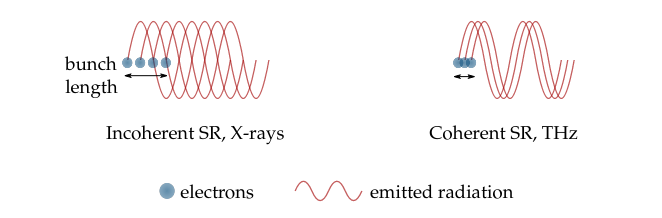
\includegraphics[width = 0.7\textwidth]{chap/02-theory/img/csr2.png}
	\caption{Placeholder \cite{rota2018}}
	\label{fig:csr}
\end{figure}

\begin{figure}[tbh]
	\centering
	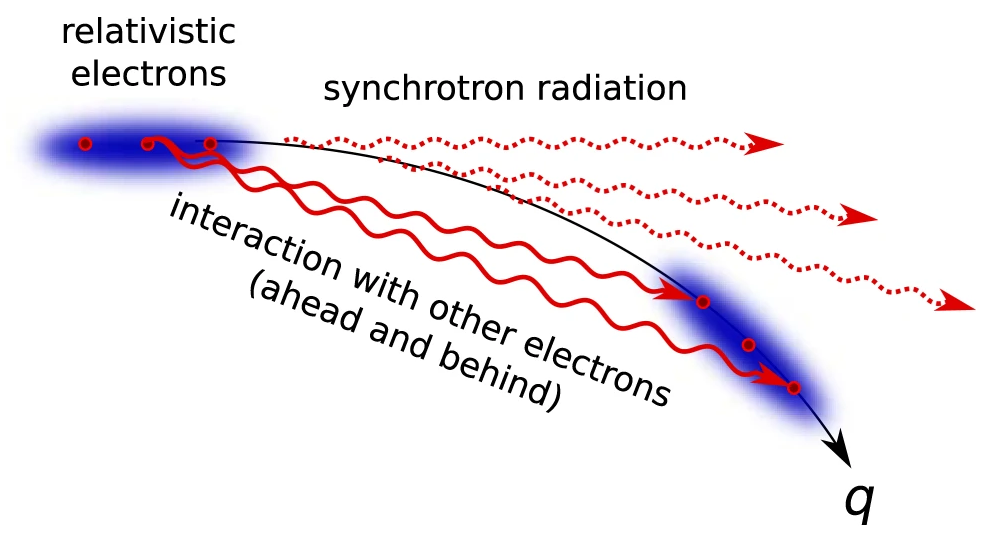
\includegraphics[width = 0.5\textwidth]{chap/02-theory/img/microbunching}
	\caption{Electrons interact with their own radiation \cite{Bielawski2019}}
	\label{fig:microBunch}
\end{figure}

\subsection{Karlsruhe Research Accelerator (KARA)(?)}
\begin{itemize}[noitemsep]
	\item Located at the Karlsruhe Institute of Technology (KIT)
	\item Up to 184 electron bunches can be filled with a distance of \SI{2}{\nano\second} (\SI{500}{\mega\hertz}) between two adjacent bunches %todo filled?
	\item Operated by the Institute of Beam Physics and Technology (IBPT)
	\item Microtron, Booster Synchrotron, and Storage Ring
\end{itemize}

\begin{table}[tbh]
	\caption{KARA characteristics}
	\label{tab:kara}
		\centering
	\begin{tabularx}{\textwidth}{Xl}
			\toprule
			Beam energy    				& $ \SI{2.5}{\giga \electronvolt}$ \\
			Circumference 	 				& $\SI{110}{\meter}$	  \\
			RF frequency    				& $\SI{499.7}{\mega \hertz}$ 	\\
			Harmonic number 				& 184	\\
			Number of RF stations 			& 2 \\
			Number of cavities per station 	& 2	\\
			Accelerating voltage 					& $\SI{1.4}{\mega \electronvolt}$ \\
			\bottomrule		
	\end{tabularx}
\end{table}
%todo why minipage? S-columns only make sense if all vars in one column have the same unit, just use a 'l' column here?
%todo maybe remove the textbf here and in all other tables (unprofessional, clutters page, etc. was auch immer)

\subsection{Beam Diagnostics at KARA}

\begin{figure}[tbh]
	\centering
	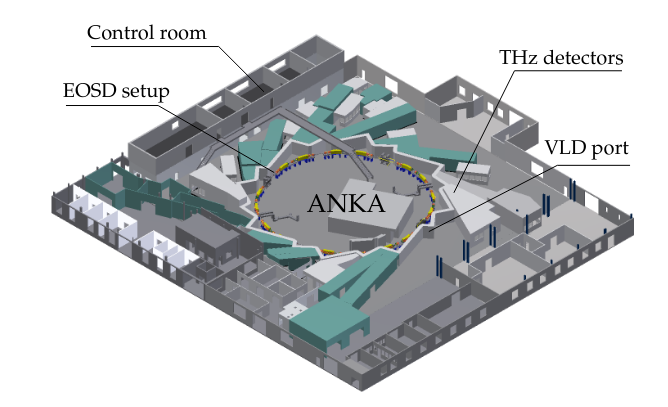
\includegraphics[width = 0.6\textwidth]{chap/02-theory/img/kara.png}
	\caption{Facility \cite{rota2018}}
	\label{fig:kara}
\end{figure}
%todo keep the figure, but remove, then redraw labels in tikz?

\newpage 
\section{Electro-Optic Techniques and Time-Stretch}
%todo what exactly do we want to measure? then introduce EO
Several \gls{eo} techniques exist, to measure THz radiation with a sub-picosecond resolution.
In this section, the techniques used in storage rings and the time-stretch technique are presented. 

\subsection{Scanning-Type Electro-Optic Sampling}
%todo what is that, one sentence
A short laser pulse (duration typically hundreds of femtoseconds) co-propagates with a THz pulse from \gls{csr} (range of picoseconds) in an \gls{eo} crystal. Due to the Pockels effect\footnote{"The Pockels effect is the name given to the occurrence of
birefringence and to the change in existing birefringence phenomena in an electric field linearly proportional to the electric
field strength." \cite{pockels}} the THz pulse causes a time dependent birefringence in the crystal.
%todo avoid direct quote
This modulates the polarization of the laser pulse.
To sample the pulse, the delay between the laser and the THz pulse is varied.
To detect the changing polarization, the polarization of the laser pulse is transformed into an intensity modulation.
A general scheme of the system is shown in \autoref{fig:scan_eo}.
For this technique a stable emission of the THz pulses is crucial, as they are not measured in one acquisition. \cite{roussel2014}
\begin{figure}[H]
	\centering
	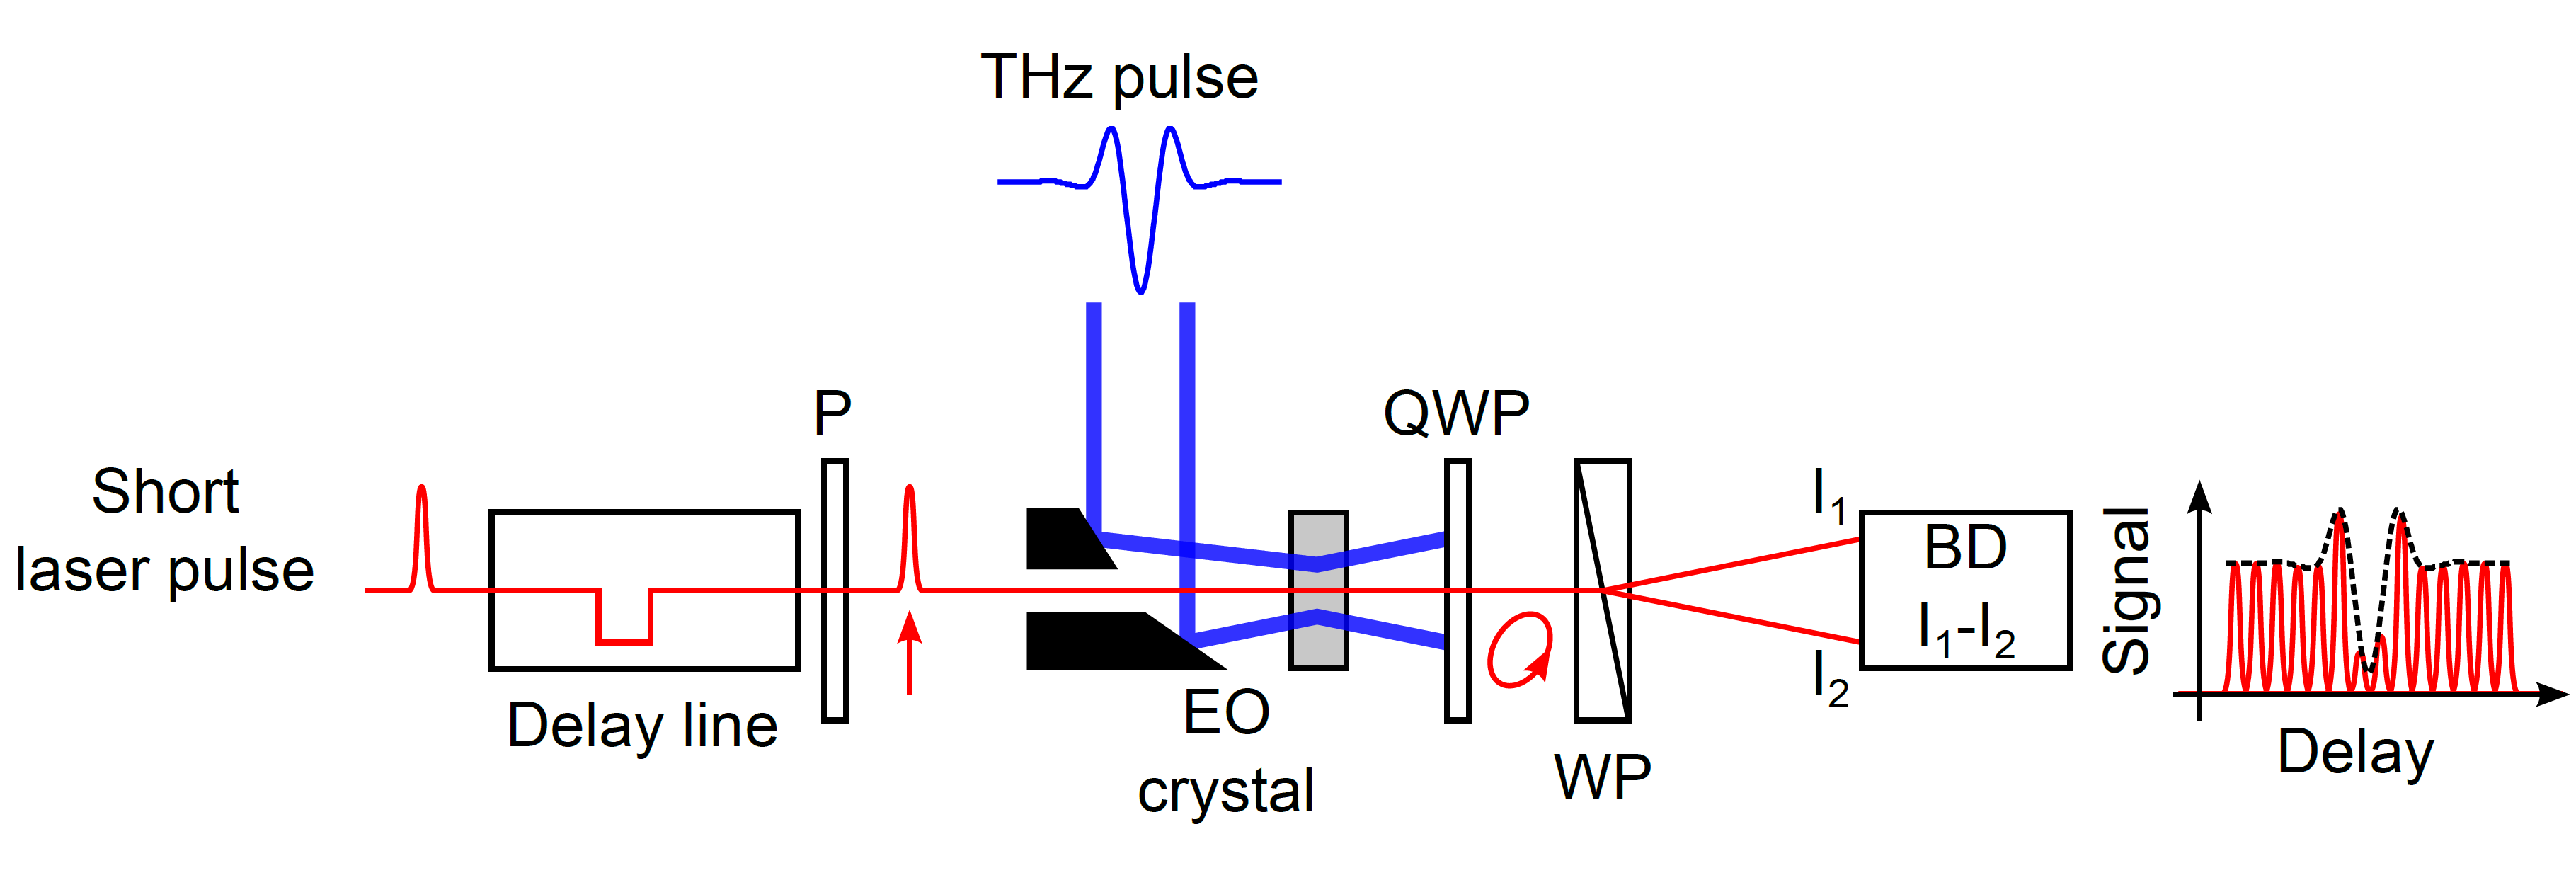
\includegraphics[width = 0.8\textwidth]{chap/02-theory/img/scanning_eo}
	\caption{Scheme of Scanning-Type Electro-Optical Sampling System \cite{roussel2014}}
	\label{fig:scan_eo}
\end{figure}

\subsection{Spectrally Resolved Electro-Optic Detection}
In contrast to the EOS, single-acquisition is possible with the spectrally resolved electro-optic detection technique. %todo EOS==EO?
The short laser pulse is first stretched to a duration similar to the Thz pulse in a dispersive material (stretcher).
In this way the pulse is chirped, meaning the instantaneous frequency of the pulse varies over time.
Together with the THz, the laser pulse propagates in a \gls{eo} crystal.
Again, the induced birefringence modulates the laser pulse, not only in time, but also in the optical spectrum.
The polarization state of the pulse is converted into an amplitude/intensity modulation.
To retrieve the THz pulse shape in time, the spectrum of the laser pulse is measured with a spectrometer. %todo what spectrometer (optical or electrical) or state model
A general scheme of the system is shown in \autoref{fig:spectral_eo}. \cite{roussel2014}

\begin{figure}[tbh]
 	\centering
 	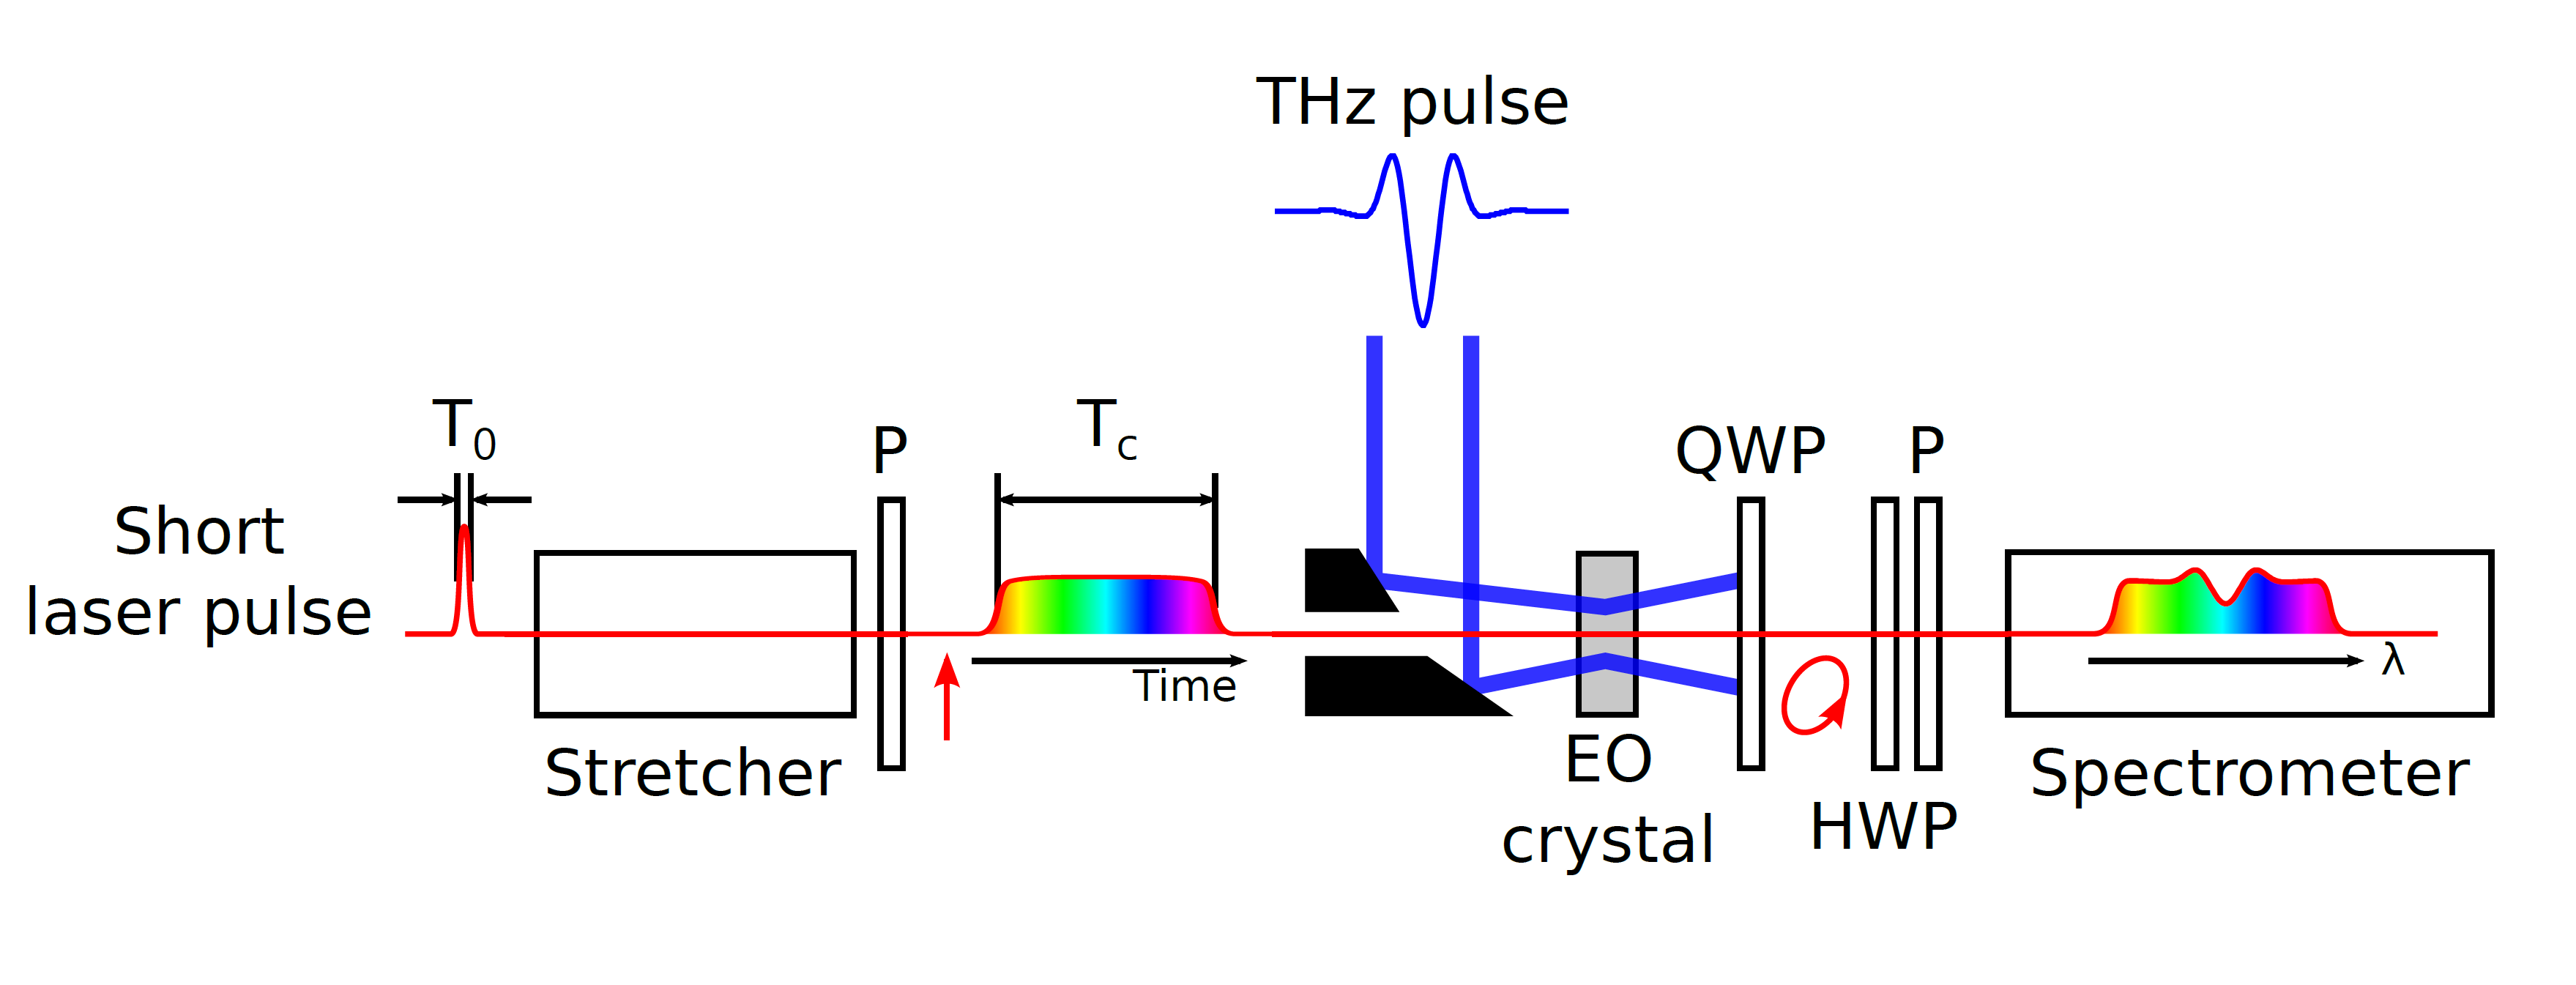
\includegraphics[width = 0.8\textwidth]{chap/02-theory/img/spectral_eo}
 	\caption{Scheme of Spactrally Encoded Electro-Optical Detection System \cite{roussel2014}}
 	\label{fig:spectral_eo}
\end{figure}

The temporal resolution of this method is limited due to the finite chirp rate
\begin{equation}
\text{chirp rate} = \frac{\text{laser bandwidth}}{\text{laser pulse duration after stretcher}}.
\end{equation}

The resolution $T_{\text{min}}$ is determined as
\begin{equation}
T_{\text{min}} = \sqrt{T_0 T_c}
\end{equation}
with the bandwidth-limited pulse duration (before stretcher) $T_0$ and the duration of the chirped laser pulse $T_c$.

\subsection{Photonic Time-Stretch Technique}
The working principle of the optic time-stretch technique can be described in two steps (see \autoref{fig:eo_ts}).
First, like in the EOSD before, a short laser pulse is propagated in a dispersive medium (optical fiber of length $L_1$). %todo EOSD?
This results in a chirped laser pulse of the duration
\begin{equation}
	T_1 = \Delta \lambda D_1 L_1
\end{equation}
with the optical bandwidth of the laser pulse $\Delta \lambda$  and the dispersion parameter $D_1$ of the fiber.
The next step is the time-to-wavelength-mapping, where a temporal intensity modulation is imprinted on the chirped pulse.
After that, the modulated chirped pulse propagates through another dispersive medium, a fiber of the length $L_2$.
In this way, the temporal modulation of the pulse is further stretched to the duration $T_2$, which is long enough for detection with photodetectors. \cite{roussel2014}

The factor, by which the pulse is slowed down, is calculated as
\begin{equation}
	M = 1 + \frac{L_1}{L_2}.
\end{equation}

\begin{figure}[tbh]
	\centering
	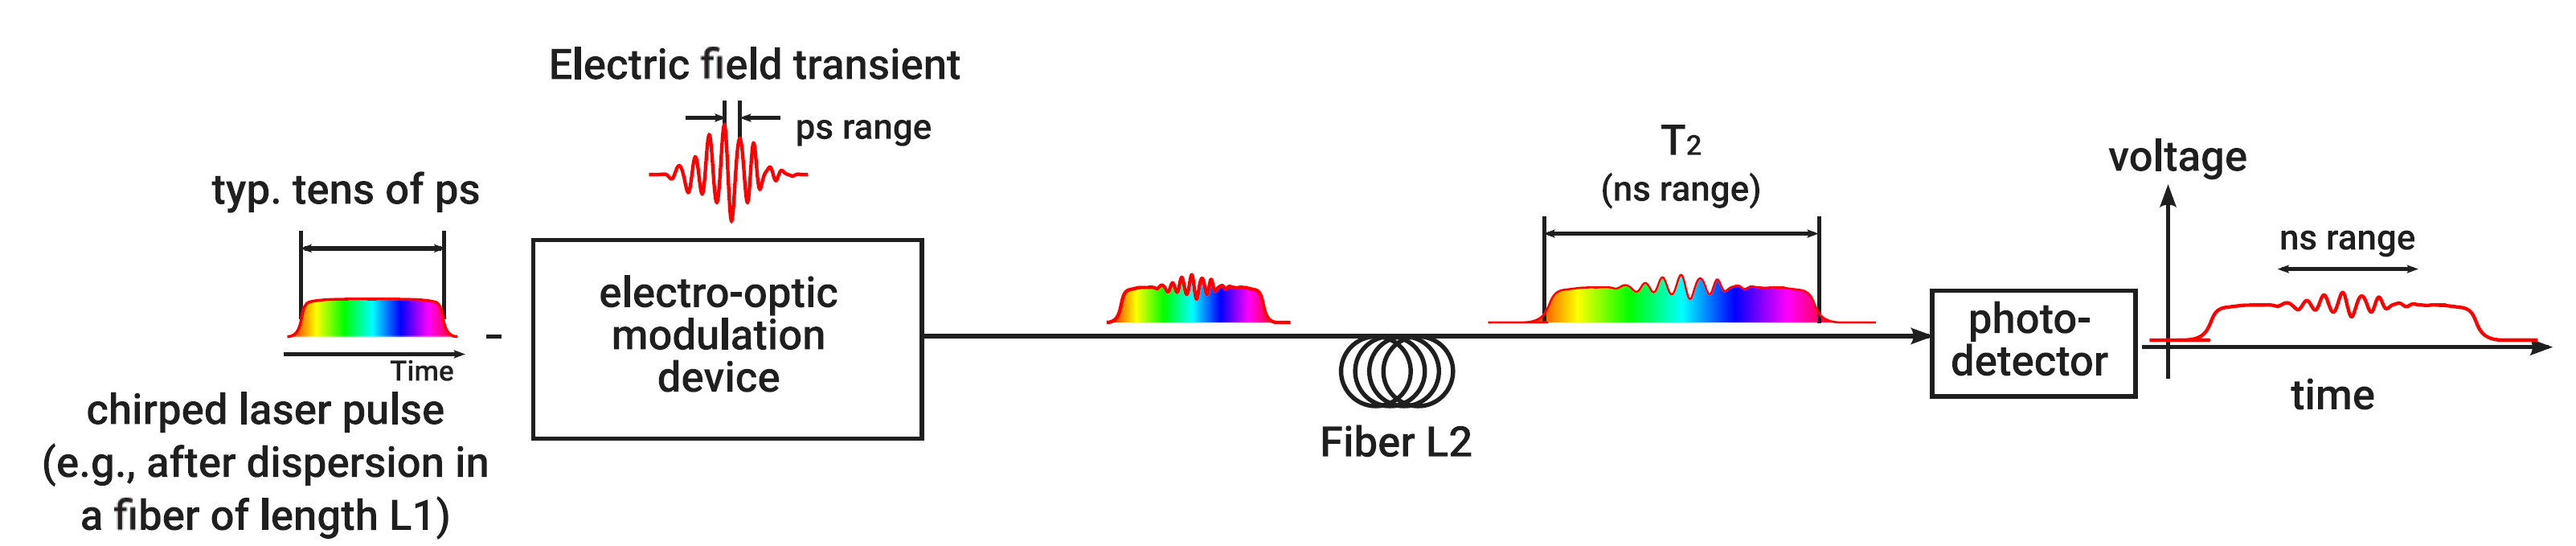
\includegraphics[width = \textwidth]{chap/02-theory/img/time_stretch.png}
	\caption{Electro-Optical Time-Stretch Technique \cite{szwaj}}
	\label{fig:eo_ts}
\end{figure}
%todo at least re-add labels in the figure with tikz, or they are too small

\subsection{Time-Stretched Spectrally-Encoded Electro-Optic detection}





\newpage
\section{Analog-To-Digital Converters}
\Glspl{adc} are used to translate analog quantities into digital signals, which can be processed by information processing, computing, data transmission and control systems. The translation can be seen as encoding a continuous-time analog input (voltage) into a series of discrete, $N$-bit words. This can be expressed as
\begin{equation}
	V_{\text{IN}} = V_{\text{FS}} \sum_{k = 0}^{N-1} \frac{b_k}{2^{k+1}} + \epsilon
\end{equation}
with $V_{\text{IN}}$ being the input voltage, $V_{\text{FS}}$ the full-scale voltage, $b_k$ the individual output bits and $\epsilon$ the quantization error. \autoref{fig:idealADC} shows the ideal transfer function of a 3-bit \gls{adc}.
\begin{figure}[H]
	\centering
	\includegraphics[width = 0.55\textwidth]{chap/02-theory/img/ideal_adc}
	\caption{Transfer function of an ideal, 3-bit \gls{adc} (redrawn from \cite{Lundberg})}
	\label{fig:idealADC}
\end{figure}
%todo Can this be combined with the other section about nyquist?
%todo ALL CAPS in the eqs?
 %todo what is an ADC, why do we need one in general?

\subsection{Sampling Theory}
An \gls{adc} samples an analog signal with a sample frequency $f_s$.
This frequency has to be chosen in such way, that the original signal can be fully reconstructed.
The \textit{Nyquist criteria} states, that in order to accurately represent a band-limited, continuous signal %todo what is B?
%todo rewrite the condition, maybe like Y(f)=0\vert_f>B/2
\begin{equation}
	y (t) \, \fourier  Y(f) \quad \text{with} \quad Y(f) = 0, \, |f| \geq \frac{B}{2}
\end{equation}
it has to be sampled with a frequency $f_s$ respecting
\begin{equation}
	f_s \geq B \quad \text{or} \quad f_s \geq 2 f_a
\end{equation}
with $f_a$ being the highest frequency contained in the signal. \cite{walt,puente2015}
%todo why not relate f_a to B?

In other words, $f_a$ must be inside of the \textit{Nyquist bandwidth}, which is the spectrum from DC to $f_s/2$. Violation of this rule leads to \textit{aliasing}.
%todo what is DC? state that in this paragraph you argue the other way around: now the sampling rate limits the signal bandwith and not the signal bandwith gouverns the samling freq

\begin{figure}[tbh]
	\centering
	\begin{subfigure}{\textwidth}
		\centering
		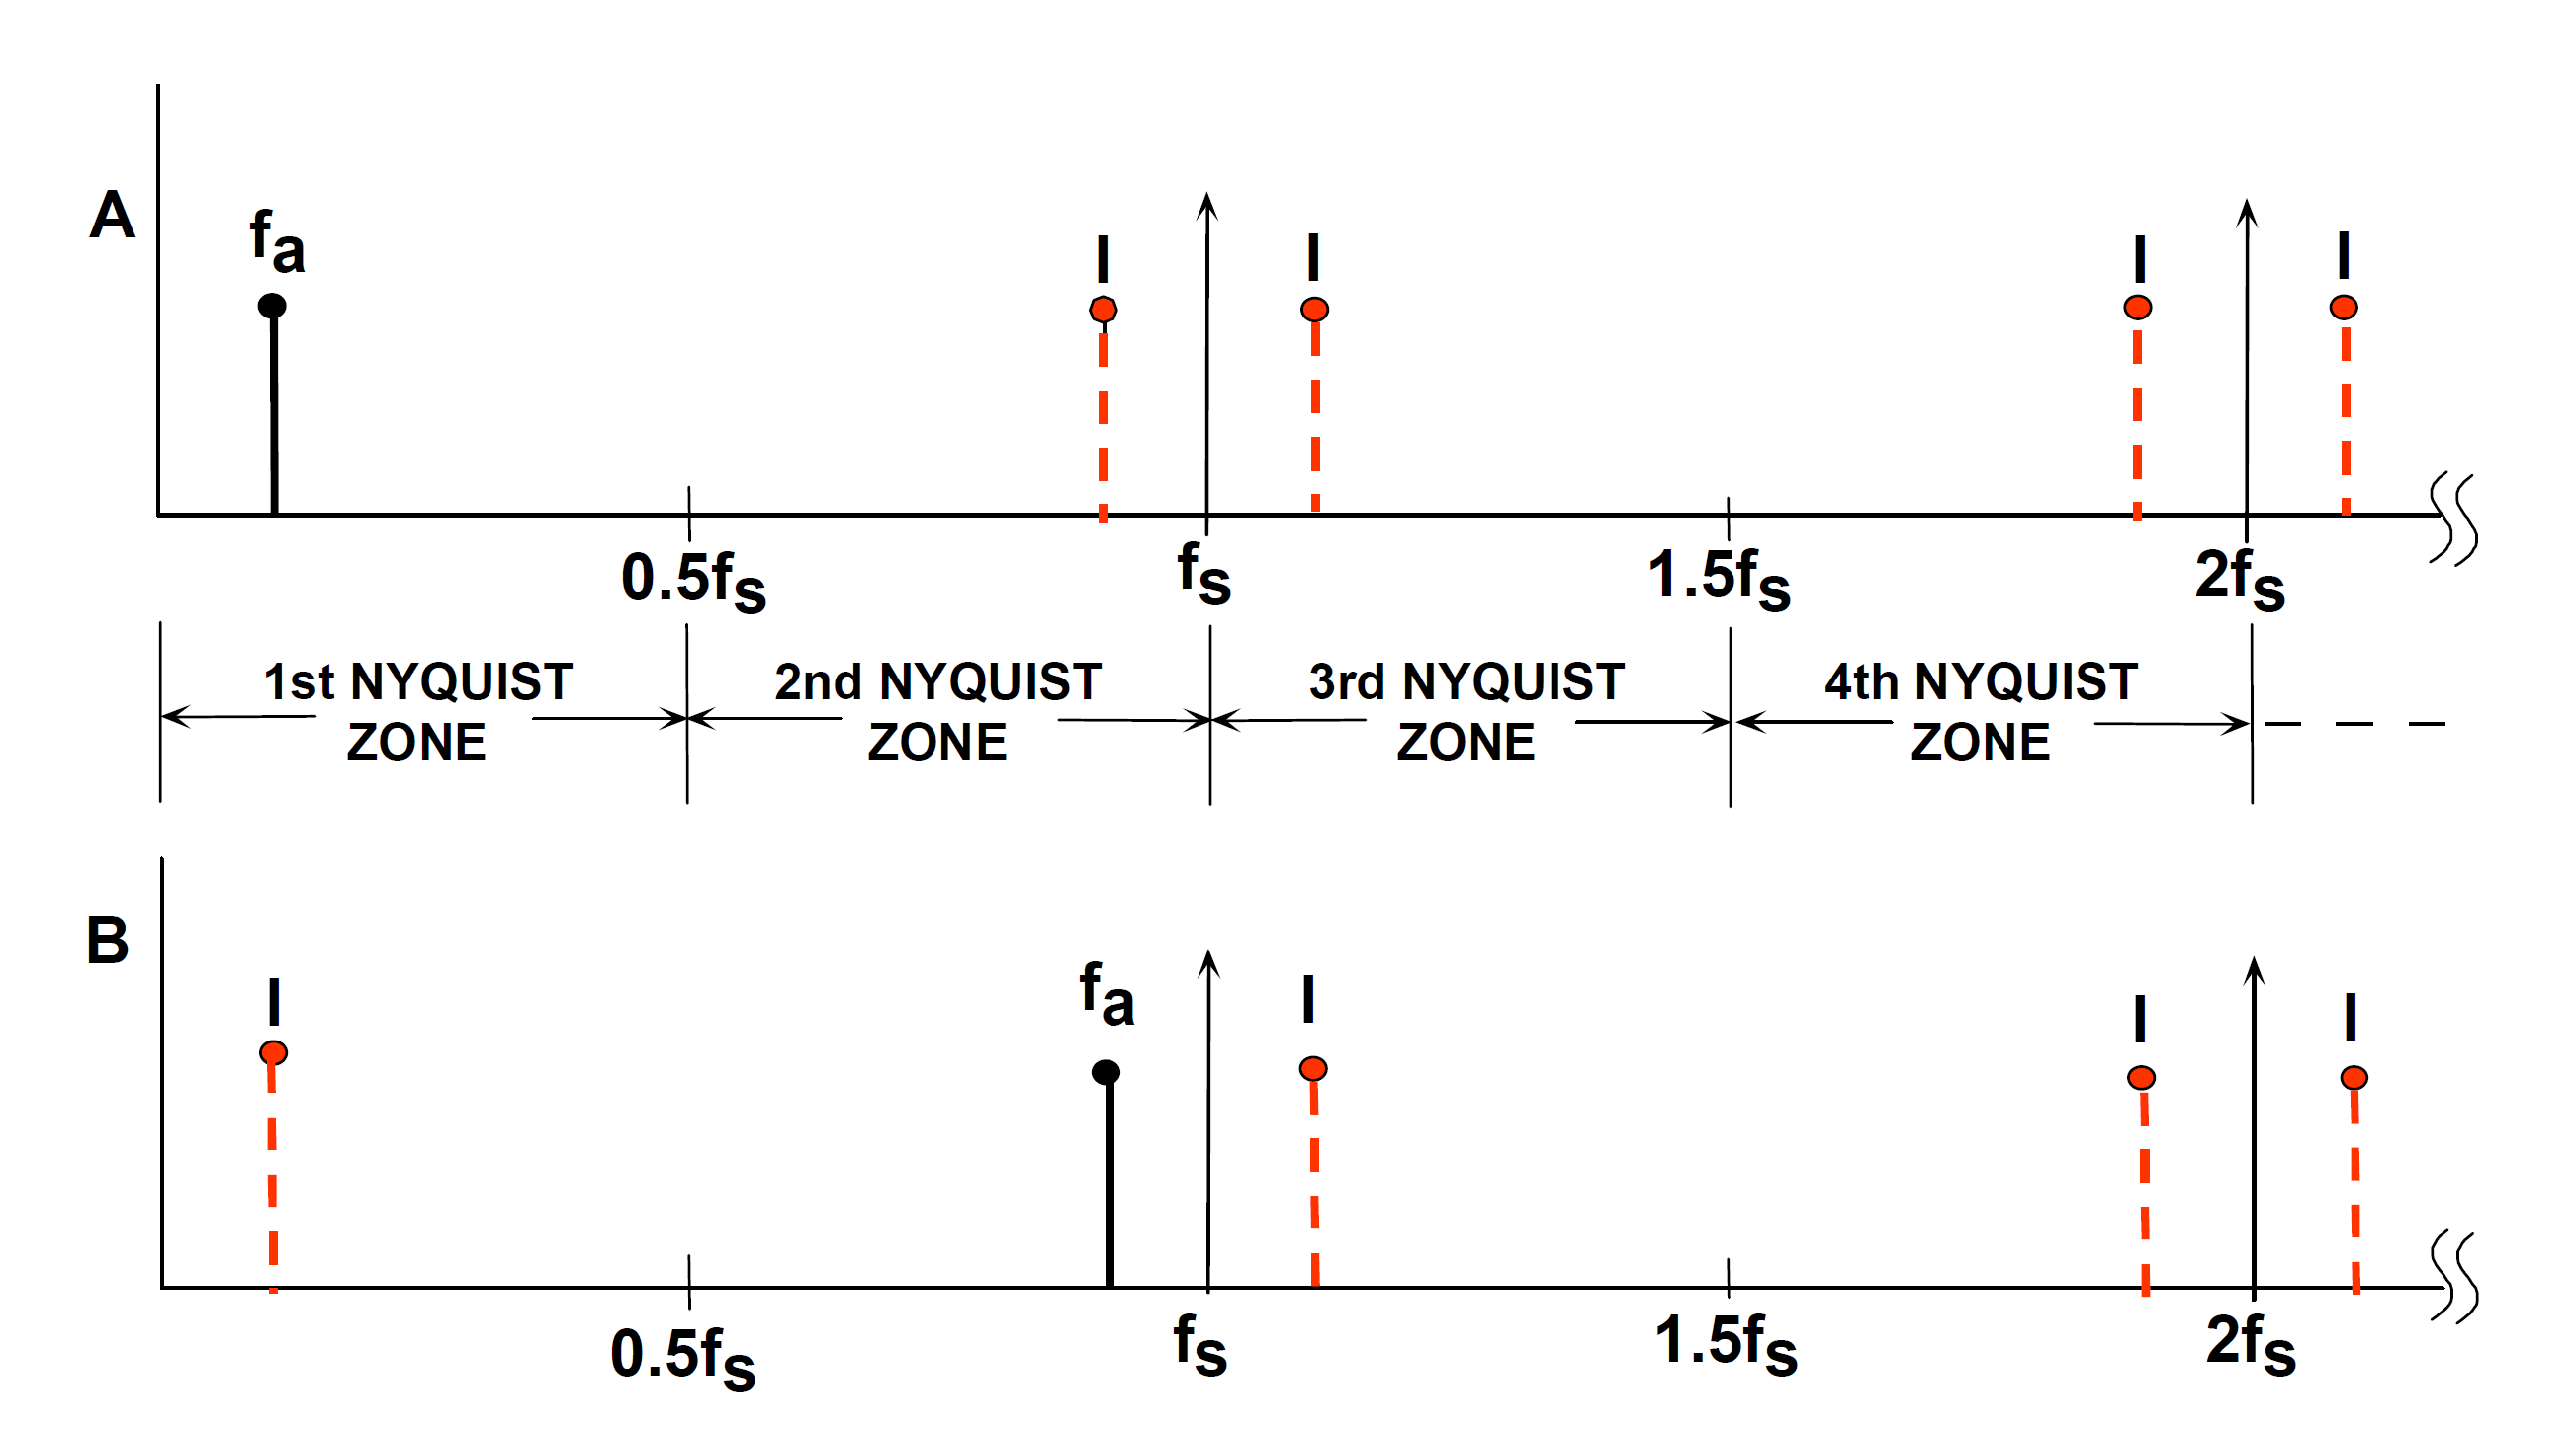
\includegraphics[width=.6\linewidth]{chap/02-theory/img/alias_f}  
		\caption{Sampling in frequency domain}
		\label{fig:alias_f}
	\end{subfigure}
	\begin{subfigure}{\textwidth}
		\centering
		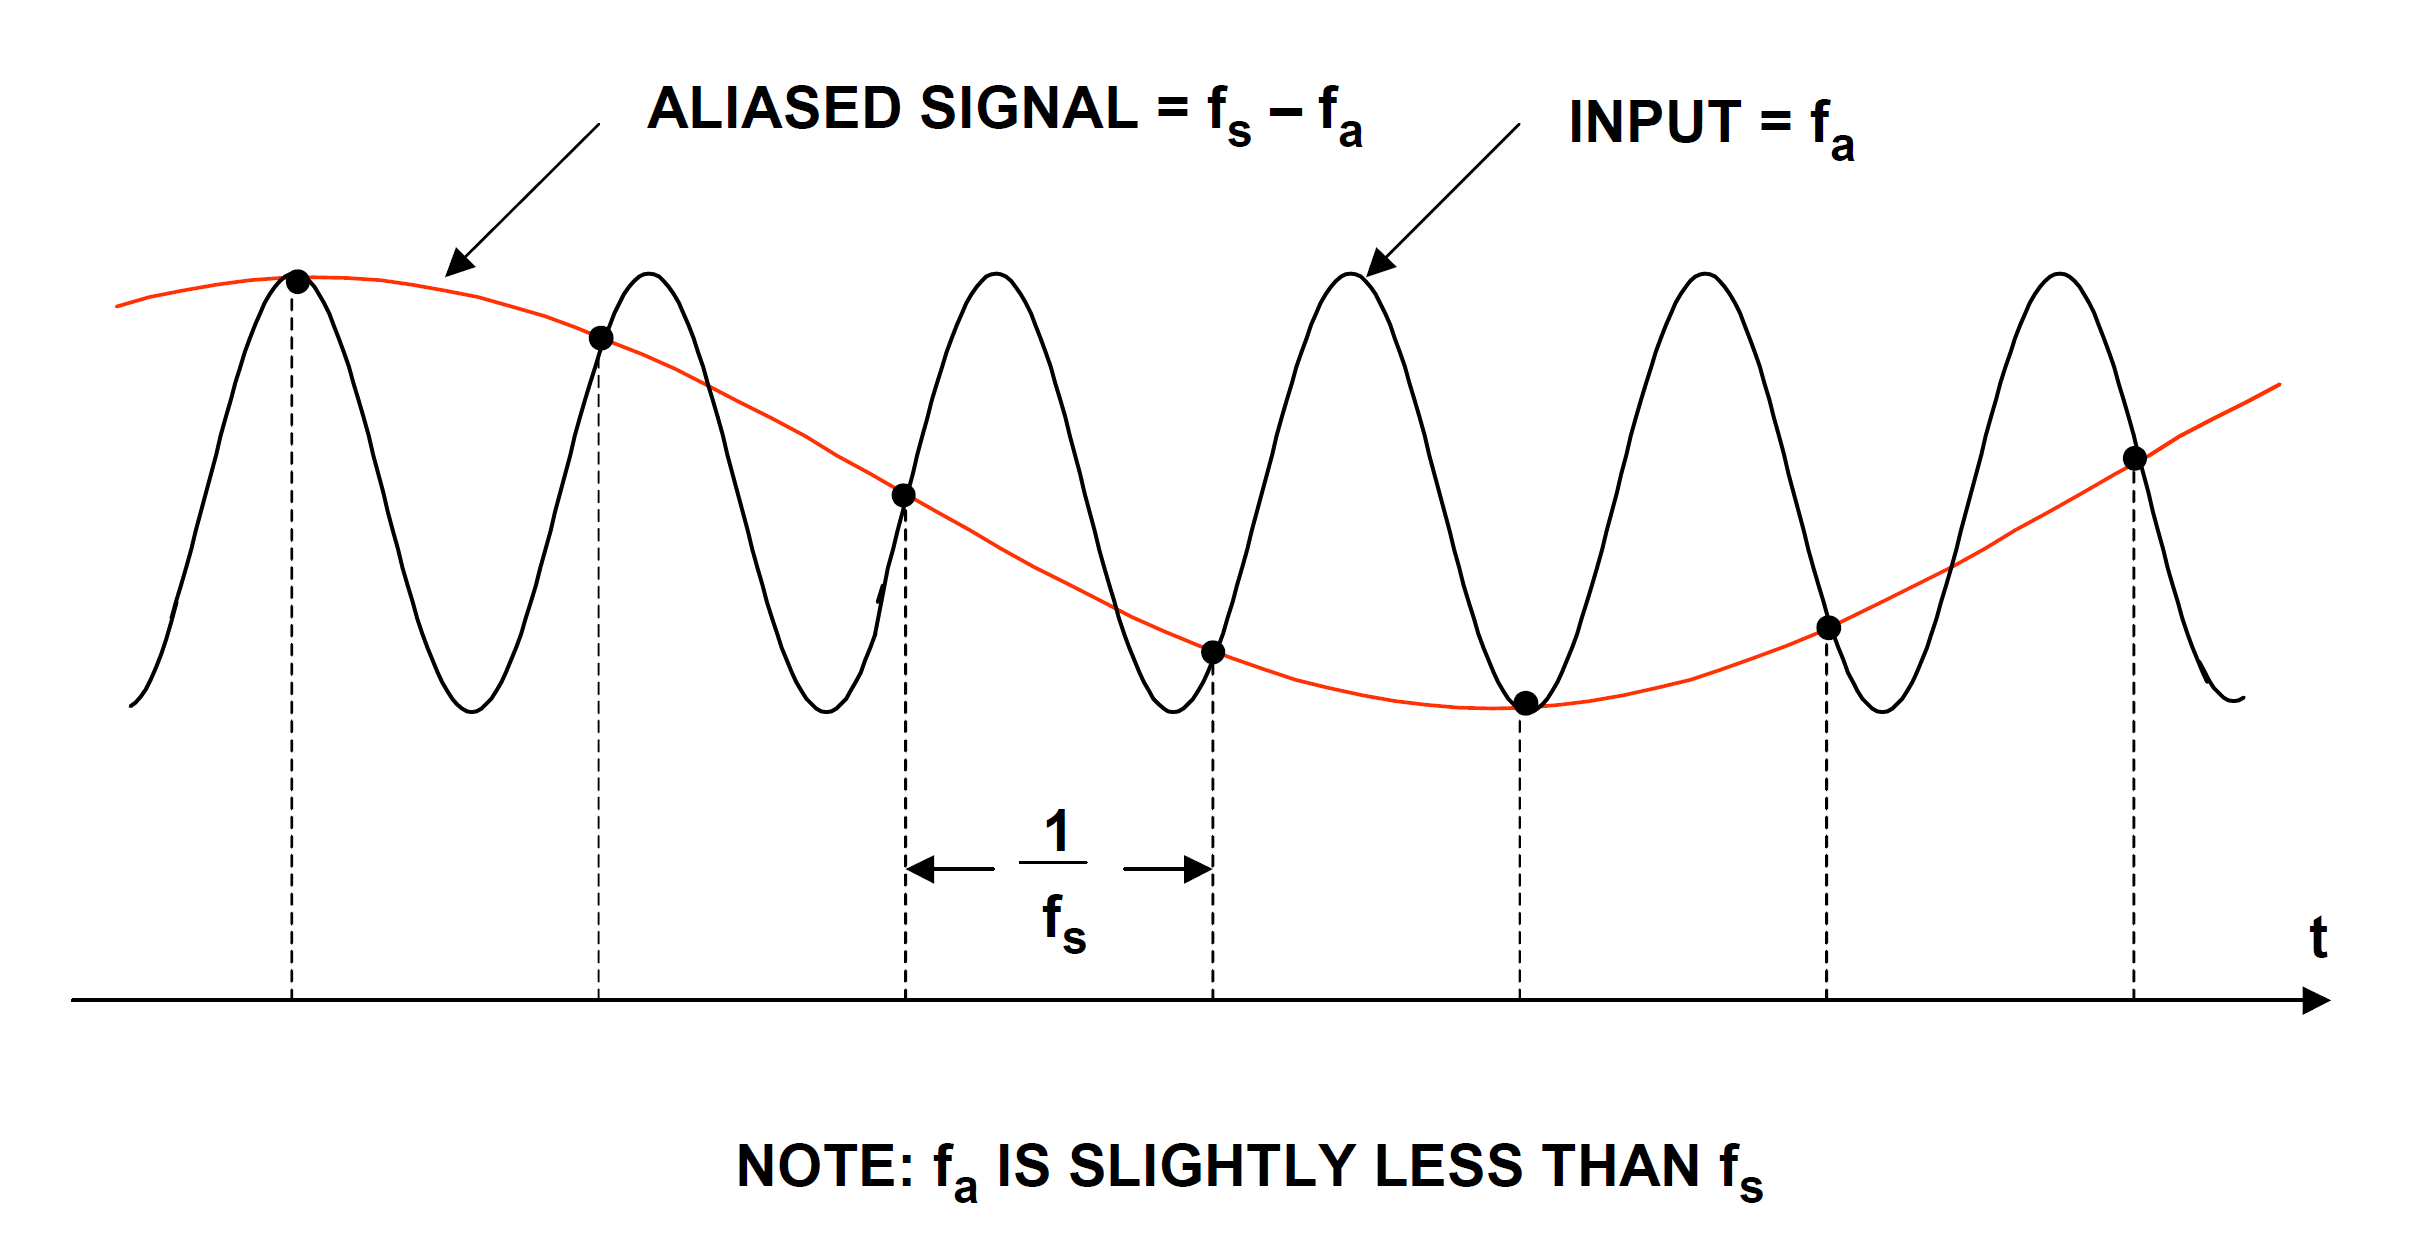
\includegraphics[width=.6\linewidth]{chap/02-theory/img/alias_t}  
		\caption{Aliasing in time domain}
		\label{fig:alias_t}
	\end{subfigure}
	\caption{Analog signal with frequency $f_a$ sampled at $f_s$ respecting (A) and not respecting (B) the Nyquist criteria. \autoref{fig:alias_t} shows the effect of case B in time domain. \cite{walt}}
\end{figure}
%todo add [] short image caption

%todo low-pass filter to get B/2<f_s? maybe


\paragraph{Sample-And-Hold-Amplifier}
\Glspl{adc} need a certain amount of time to sample the input signal.
If the level of the analog signal changes by more than one \gls{lsb} during this period, this can result in large errors in the output signal.
Therefore, so called \gls{sha} are used in front of the \gls{adc} to hold the input level constant for the needed amount of time.
The \gls{adc} sampling time needs to be timed in such way, that the analog-to-digital conversion falls into the hold period of the \gls{sha} and does not exceed into the sample period, for example like shown schematically in the diagram below. Thus, the upper frequency limitation is not determined by the \gls{adc} itself, but rather by the aperture jitter, bandwidth, distortion, etc. of the \gls{sha}. \cite{walt}



\begin{figure} [tbh]
	\centering
	\tikzexternaldisable
	\begin{tikztimingtable}
		[%
		timing/dslope=0.1,
		timing/name/.style={font=\sffamily\normalsize},
		timing/d/text/.style={font=\sffamily\normalsize},
		grayz/.style={timing/z/.append style={gray}},
		timing/n/.style={rectangle},
		timing/metachar={{K}[2]{#1l !{++(0,+.5\yunit)} N[rectangle,scale=.6]{\shortstack{#2}} !{++(0,-.5\yunit)} #1l}},
		timing/metachar={{J}[2]{#1h !{++(0,-.5\yunit)} N[rectangle,scale=.6]{\shortstack{#2}} !{++(0,+.5\yunit)} #1h}},
		]
		SHA & 1H 8K{HOLD} 8J{SAMPLE} 8K{HOLD} 3H\\
		Sampling & 5S A 15S A                    \\
	\end{tikztimingtable}
	\tikzexternalenable
\end{figure}
%todo why not save this as .tikz file and include it as a normal figure with caption?

In addition to the \gls{sha}, there is also the \gls{tha}.
Instead of a sample period, the \gls{tha} has a track period, where the output of the amplifier tracks the input signal (see also \autoref{fig:tha}).
When switching to hold mode, the signal at this instant is held. This is opposed to the \gls{sha}, where the output during sample mode is actually not defined and is set to the value of the input signal, only when switching into hold mode.
%todo explanation a bit confusing. use another timing diagram?

\begin{figure}[tbh]
	\centering
	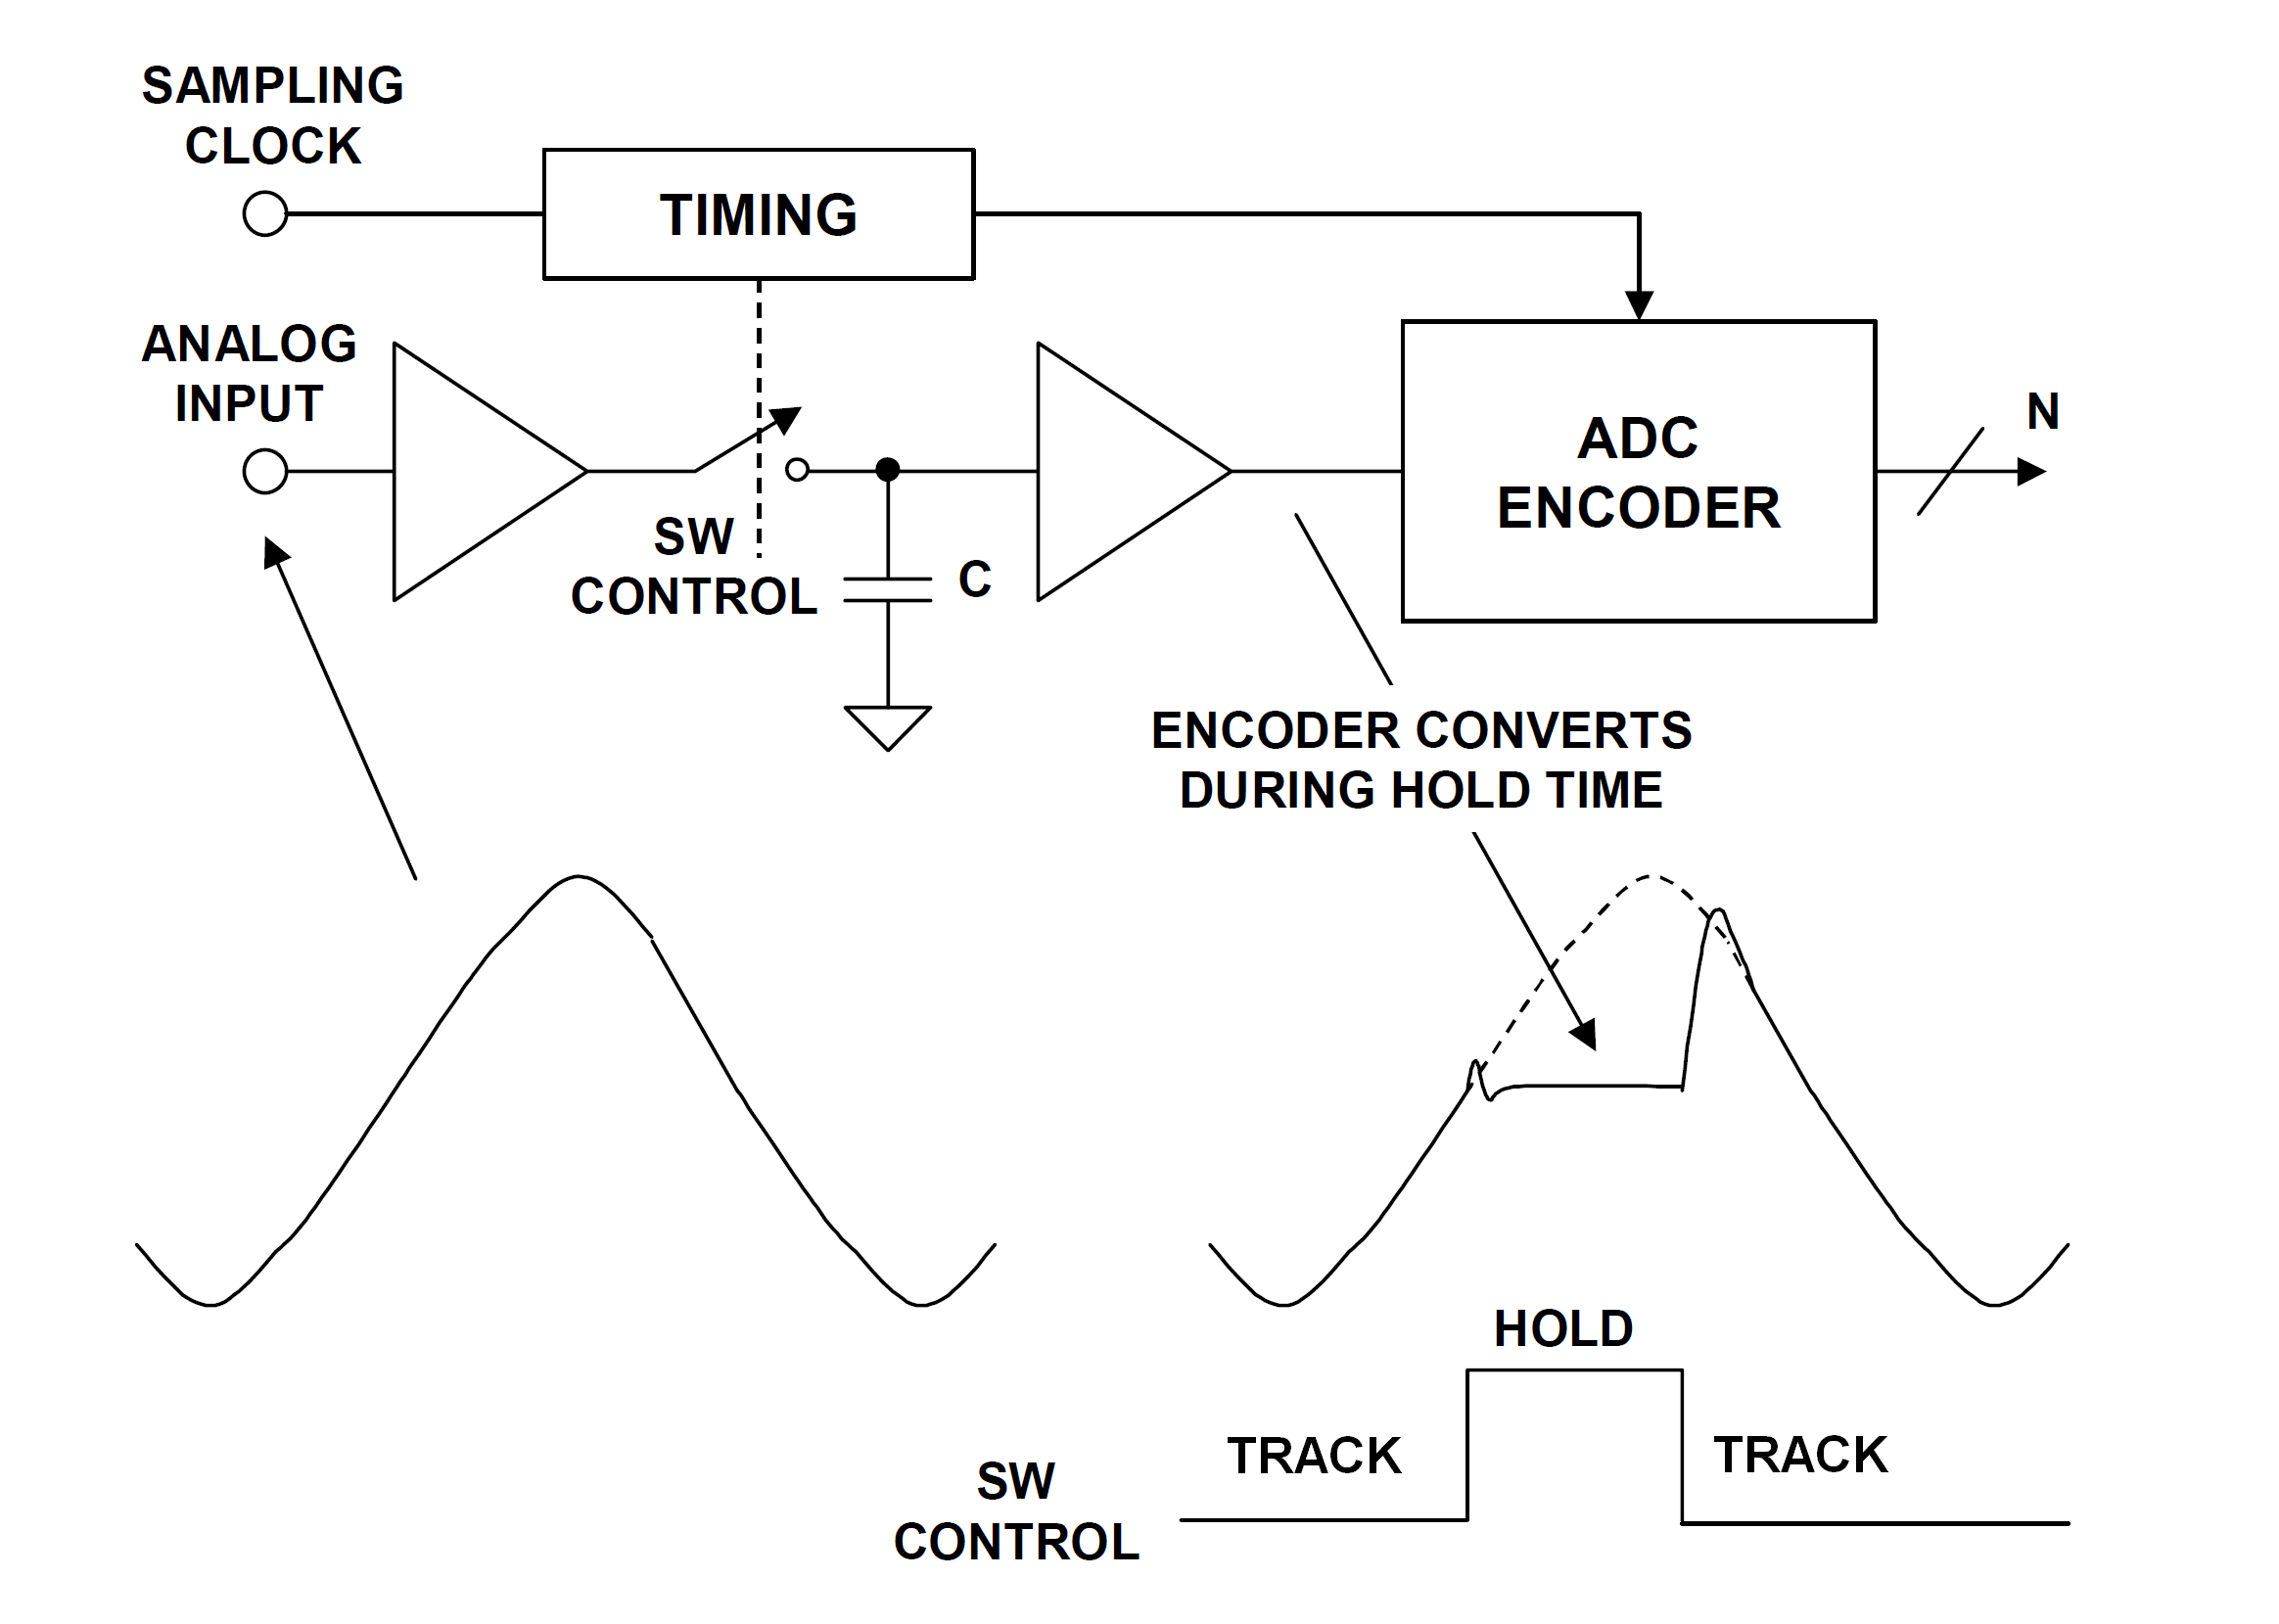
\includegraphics[width = 0.5\textwidth]{chap/02-theory/img/tha}
	\caption{Track-And-Hold-Amplifier schematic and principle \cite{walt}}
	\label{fig:tha}
\end{figure}

\subsection{Characteristics of Analog-To-Digital-Converters}



For an ideal converter, the number of bits would be sufficient to fully characterize it.
Real \glspl{adc} however differ from the ideal behavior by introducing static and dynamic imperfections.
Different applications have different requirements, which leads to a number of specifications. These can be divided into three categories \cite{Lundberg}:
\begin{itemize}[noitemsep]
	\item Static parameters
	\item Frequency-domain dynamic parameters
	\item Time-domain dynamic parameters
\end{itemize}
This section provides an overview of these figures of merit. Which of these are needed to specify the necessary performance of the \gls{adc} has to be chosen for each application accordingly.


\subsubsection{Static parameters}
\textit{Static parameters} are specifications, which can be measured at low speed/DC. 
\paragraph{Accuracy}
\textit{Accuracy} is the total error at a known voltage, which includes:
\begin{itemize}[noitemsep]
	\item Quantization error
	\item Gain error
	\item Offset error
	\item Non-linearities
\end{itemize}

\paragraph{Resolution}
\textit{Resolution} is the number of bits $N$ of the \gls{adc}. Depending from the resolution are the size of the \gls{lsb}, which in its turn determines the dynamic range, code widths and quantization error.

\paragraph{Dynamic Range}
Ratio between smallest possible output (\gls{lsb} voltage) and the largest possible output (full-scale voltage). It can be calculated as
\begin{equation}
	20 \log 2^{N} \approx 6N.
\end{equation}


\paragraph{Offset and Gain Error}
The \textit{offset error} is the deviation of the first transition voltage from the ideal $1/2$ \gls{lsb}. \textit{Gain Error} defines the deviation of the slope of the line going through the zero and full-scale point of the transfer function. These errors can easily be corrected by calibration. Refer to \autoref{fig:offsetErr}

\begin{figure}[H]
	\centering
	\includegraphics[width = 0.55\textwidth]{chap/02-theory/img/offset_err.tikz}
	\caption{Offset and Gain Error in the \gls{adc} characteristic. Notice the difference between the ideal, dotted line}
	\label{fig:offsetErr}
\end{figure}


\paragraph{Integral and Differential Non-linearity Distortion} 
\textit{Integral non-linearity} in the transfer function of data converters results from the integral non-linearities of the front-end, \gls{sha} and also the \gls{adc} itself.
These non-linearities depend on the input signal amplitude.
distance of the code centers in the A/D converter characteristic from the ideal line
\textit{Differential non-linearities} stem exclusively from the encoding process in the \gls{adc}.
They not only depend on the input signal amplitude, but also on the positioning along the transfer function.
The deviation of the code transition widths from the ideal width
of 1 \gls{lsb}.

\subsubsection{Dynamic performance}
\paragraph{Frequency-Domain}
\begin{itemize}
	\item SINAD
	\item ENOB
	\item SFDR
	\item Total Harmonic Distortion
	\item Intermodulation Distortion
	\item Effective Resolution Bandwidth
	\item Full-Power Bandwidth
	\item Full-Linear Bandwidth
\end{itemize}
\paragraph{Time-Domain}
\begin{itemize}
	\item Aperture Delay
	\item Aperture Jitter
	\item Transient Response
	\item Overvoltage Recovery
\end{itemize}

\subsubsection{Quantization Noise}
Even in an ideal $N$-bit converter there will be errors during the quantization, which behave like noise.
The reason is that each $N$-bit word represents a certain range of analog input values, which is 1 \gls{lsb} wide (\textit{code width}) and centered around a \textit{code center} (see \autoref{fig:idealADC}) \cite{Lundberg}.
The input voltage is always assigned to the code of the nearest code center. 
This means that there will always be a difference between the code center and the actual input.
The difference betweenand the analog input $x(t)$ and its quantized signal $x_q(t)$ is called the \textit{quantization error}.
For an equidistant quantization it is
\begin{equation}
\left| e_q(t) \right| = \left| x(t) - x_q(t) \right| \leq \frac{q}{2}
\end{equation}
with $x_q(t)$ being the quantized/discrete signal, $x(t)$ the input signal and $q$ the width of the quantization stage. \cite{puente2015}
%todo maybe push the explanations for x and x_q higher up, like 'for a signal x(t) and its quantized signal x_q(t)[...]'

Assuming the error voltage uncorrelated and uniformly distributed, the theoretical (maximum) Signal-To-Noise-Ratio (SNR) of this \textit{quantization noise} can be calculated. In the time domain, the quantization error can be approximated with a sawtooth signal \cite{walt}:
\begin{equation}
e_q(t) = st, \quad -\frac{q}{2s} < t < \frac{q}{2s} 
\end{equation}
%todo why sawtooth? what is 's'? cite?

\begin{figure}[tbh]
	\centering
	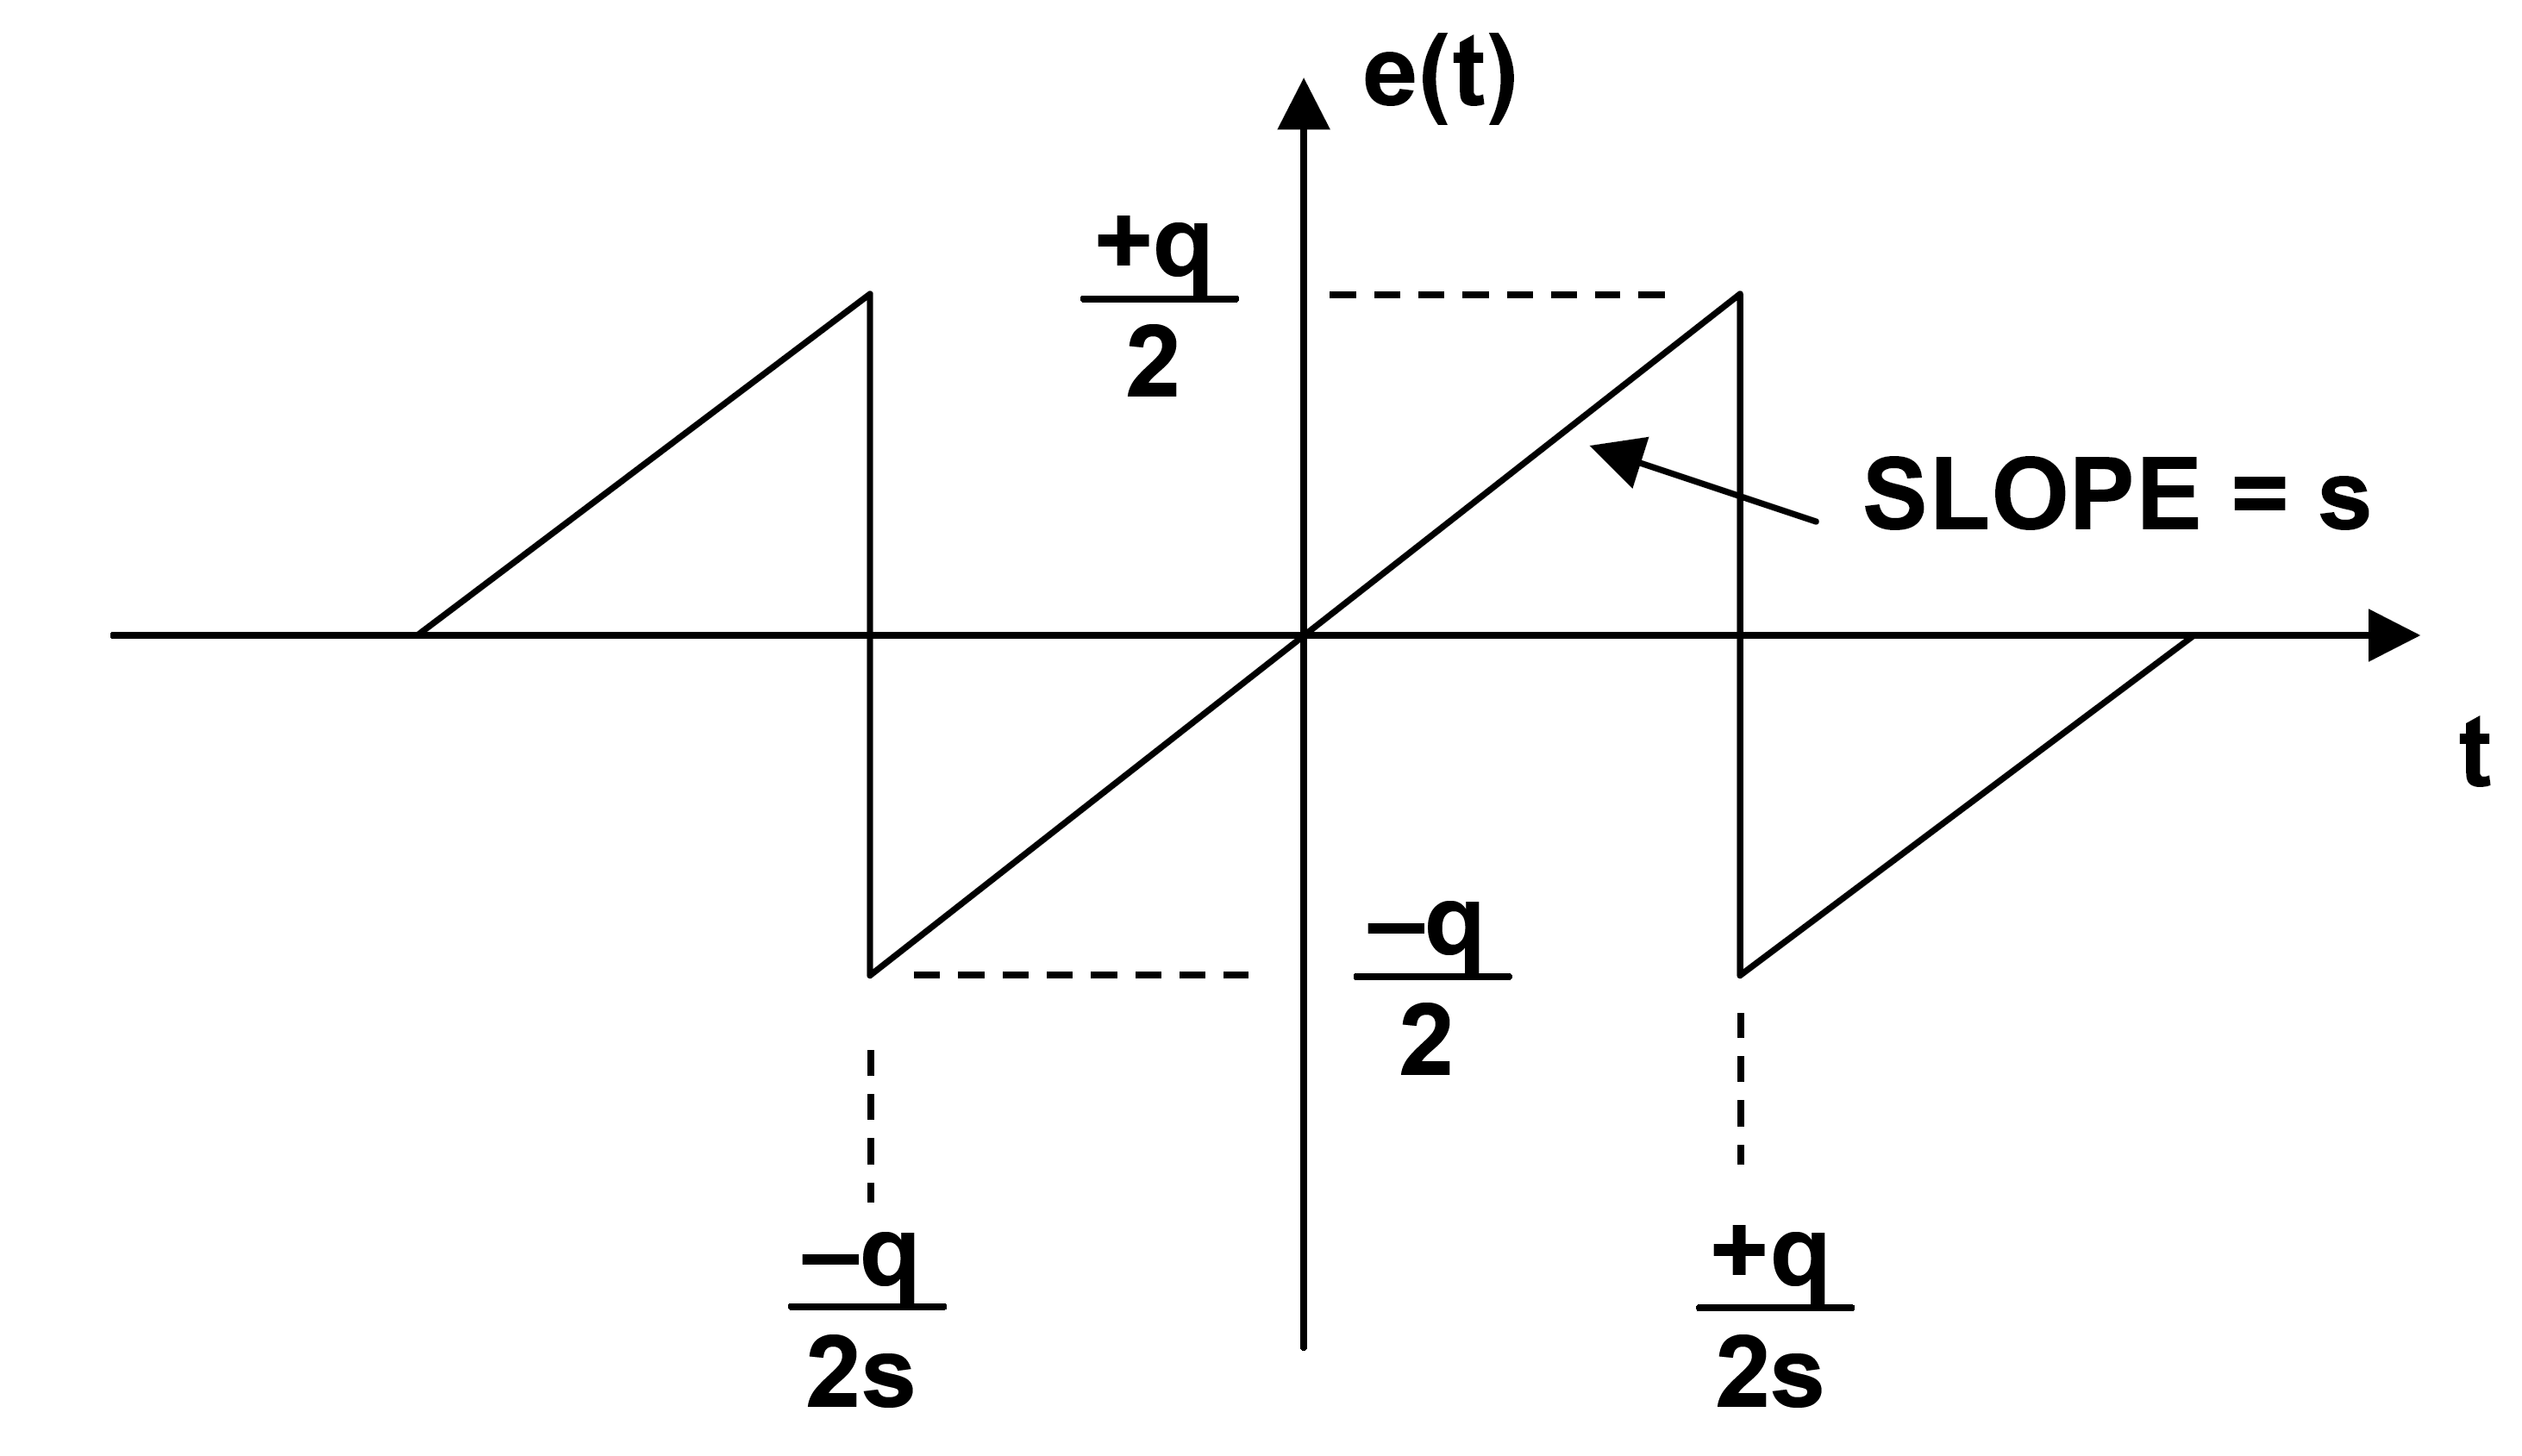
\includegraphics[width = 0.5\textwidth]{chap/02-theory/img/quantization_error.tikz}
	\caption{Quantization noise as function of time (redrawn from \cite{walt})}
	\label{fig:eq}
\end{figure}

%todo how does e relate to e_q?

The power of the quantization noise, which is assumed to be uncorrelated and broadband, can be calculated as the mean-square of $e_q(t)$:
\begin{equation}
P_\text{QN} = e_{\text{rms}}^{2} = \overline{e^{2}(t)} = \frac{s}{q}\int_{-q/2s}^{+q/2s} (st)^{2} dt = \frac{s^3}{q} \left[ \frac{t^3}{3}\right]_{-\frac{q}{2s}}^{+\frac{q}{2s}} = \frac{q^2}{12}
\end{equation}

To calculate the maximal SNR of an ideal converter, a full-scale input sine wave is assumed:
\begin{equation}
u(t) = u_s \sin(2\pi f t) = \frac{2^{N}q}{2}\sin(2\pi f t)  = 2^{N-1}q \sin(2\pi f t)
\end{equation}
With the effective value of the signal amplitude
\begin{equation}
u_{\text{eff}} = \frac{u_s}{\sqrt{2}} = \frac{2^{N-1}q}{\sqrt{2}}
\end{equation}
and the quantization noise power, the SNR can be calculated as
\begin{equation}
\text{SNR} = \frac{P_{\text{signal}}}{P_{\text{noise}}} = \frac{u_{\text{eff}}^{2}}{e_{\text{rms}}^{2}} = \frac{2^{2N-2}q^2/2}{q^2/12} = 2^{2N} \cdot 1.5.
\end{equation}

Using the unit Decibel, this can be expressed as (see \cite{puente2015,walt})
\begin{equation}
\text{SNR}|_{\text{dB}} = 10\log\left(2^{2N}\cdot 1.5\right) = 6.02 N + 1.76.
\end{equation}









In an \glspl{adc} (with built-in \gls{sha}) there are a couple of sources, which introduce noise and distortion:
\begin{itemize}
	\item \textbf{Input Stage:} Wideband noise, nonlinearity and bandwidth limitation
	\item \textbf{\gls{sha}:} Nonlinearity, aperture jitter\footnote{\textit{Aperture jitter} is the sample-to-sample variation in aperture delay, with \textit{aperture delay} meaning the time, which is needed by the \gls{sha} to disconnect the holding capacitor from the input buffer.} and bandwidth limitation
	\item \textbf{\gls{adc}:} Quantization noise, integral and differential nonlinearity
\end{itemize}
In the following the most important specifications are described, which are used to characterize the performance of \glspl{adc}.



\paragraph{Equivalent Input Referred Noise}
Internal circuits of wideband \glspl{adc} produce rms noise due to resistor and thermal ("$kT/C$") noise, which is also present for DC signals. Therefore, the output of the \gls{adc} is a distribution of codes which is centered around the value of a DC input. For measuring the value of the noise, the \gls{adc} input is grounded, or held at a specific DC value, and a large amount of samples is collected and plotted as a histrogram. The noise is approximately Gaussian, thus the stndard deviation can easily be calculated.

\paragraph{Noise-Free Code Resolution}
The input referred noise described above determines the \textit{noise-free code resolution}, which is the number of bits, beyodn which it is not possible to resolve individual codes.
\cite{walt}


\subsection{Interleaving}

\begin{itemize}
\item Net sample rate
\item Interleaving Spurs
\end{itemize}

\cite{mangrob}




\newpage
\section{RF/Microwave Design Basics}

\subsection{General Techniques/Strategies?}

\subsection{Coplanar Waveguides}
\paragraph{Surface Coplanar Waveguide with Ground}  
\begin{figure}[!htbp]
	\centering
	\begin{tikzpicture}
	\filldraw[color=black, fill=black] (0,0.7) rectangle ++(9,0.3) node[pos=.5](gnd){};
	\filldraw[color=black, fill=gray!20] (0,1) rectangle ++(9,2) node[pos=.5]{\(\varepsilon_r\)};
	\filldraw[color=black, fill=black] (0,3) rectangle ++(2,.2) node[pos=.5](GND1){};
	\filldraw[color=black, fill=black] (3,3) rectangle ++(1,.2) node[pos=.5](cond1){};
	\filldraw[color=black, fill=black] (5,3) rectangle ++(1,.2) node[pos=.5](cond2){};
	\filldraw[color=black, fill=black] (7,3) rectangle ++(2,.2) node[pos=.5](GND2){};
	\draw[>=triangle 45, <->] (-0.5,1) -- (-0.5,3) node[pos=.5,anchor=east](){\(h\)};
	\draw[>=triangle 45, <->] (2,4) -- ++(1,0) node[pos=.5,anchor=south](){\(d\)};
	\draw[>=triangle 45, <->] (3,3.8) -- ++(1,0) node[pos=.5,anchor=south](){\(w\)};
	\draw[>=triangle 45, <->] (4,3.6) -- ++(1,0) node[pos=.5,anchor=south](){\(s\)};

	\draw[>=triangle 45, ->] (10,4) -- (10,3.2) node[pos=.5,anchor=west](){\(t\)};
	\draw[>=triangle 45, ->] (10,2.2) -- (10,3) node[pos=.5,anchor=west](){};
	
	\draw[decorate,decoration={zigzag,segment length=10mm, amplitude=1mm},double, double distance = 8.9pt, white] (9,0) -- (9,4);
	\draw[decorate,decoration={zigzag,segment length=10mm, amplitude=1mm},double, double distance = 8pt, white] (0,-0.5) -- (0,4);
	\draw[dashed] (0.1,1) -- (-1,1);
	\draw[dashed] (0.2,3) -- (-1,3);
	\draw[dashed] (8,3.2) -- (10,3.2);
	\draw[dashed] (8,3) -- (10,3);
		
	\end{tikzpicture}
	\caption{Edge-Coupled Coplanar Waveguide}
	\label{fig:eccw_geometry}
\end{figure}

The corresponding equations are \cite[~p197-198]{wadell}: 
\begin{equation}
	Z_{0,o} = \frac{\eta_0}{\sqrt{\epsilon_{eff,o}}} \left( \frac{1.0}{2.0 \frac{K(k_o)}{K'(k_o)} + \frac{K(\beta_1)}{K'(\beta_1)}}\right)
\end{equation}    

\begin{equation}
	Z_{0,e} = \frac{\eta_0}{\sqrt{\epsilon_{eff,e}}} \left( \frac{1.0}{2.0 \frac{K(k_e)}{K'(k_e)} + \frac{K(\beta_1 k_1)}{K'(\beta_1 k_1)}}\right)
\end{equation} 


\begin{equation}
	\epsilon_{eff,o} = \frac{2.0 \epsilon_r \frac{K(k_o)}{K'(k_o)} + \frac{K(\beta_1)}{K'(\beta_1)}}{2.0 \frac{K(k_o)}{K'(k_o)} + \frac{K(\beta_1)}{K'(\beta_1)}}
\end{equation}

\begin{equation}
	\epsilon_{eff,e} = \frac{2.0 \epsilon_r \frac{K(k_e)}{K'(k_e)} + \frac{K(\beta_1 k_1)}{K'(\beta_1 k_1)}}{2.0 \frac{K(k_e)}{K'(k_e)} + \frac{K(\beta_1 k_1)}{K'(\beta_1 k_1)}}
\end{equation}

Where

\begin{equation}
	k_o = \Lambda \frac{-\sqrt{\Lambda^2 - t_c^2} + \sqrt{\Lambda^2 - t_B^2}}{t_B\sqrt{\Lambda^2 - t_c^2} + t_c \sqrt{\Lambda^2 - t_B^2}}
\end{equation}

\begin{equation}
	k_e = \Lambda' \frac{-\sqrt{\Lambda'^2 - t_c'^2} + \sqrt{\Lambda'^2 - t_B'^2}}{t_B'\sqrt{\Lambda'^2 - t_c'^2} + t_c' \sqrt{\Lambda'^2 - t_B'^2}}
\end{equation}


\begin{equation}
	\Lambda = \frac{\sinh^2 \left( \frac{\pi (s/2.0 + w + d)}{2.0 h} \right) }{2}
\end{equation}

\begin{equation}
	t_c = \sinh^2 \left( \frac{\pi (s/2.0 + w)}{2.0 h} \right) - \Lambda
\end{equation}

\begin{equation}
	t_B = \sinh^2 \left( \frac{\pi s}{4.0 h} \right) - \Lambda
\end{equation}


\begin{equation}
	\Lambda' = \frac{\cosh^2 \left( \frac{\pi (s/2.0 + w + d)}{2.0 h} \right) }{2}
\end{equation}

\begin{equation}
	t_c' = \sinh^2 \left( \frac{\pi (s/2.0 + w)}{2.0 h} \right) - \Lambda' + 1.0
\end{equation}

\begin{equation}
	t_B' = \sinh^2 \left( \frac{\pi s}{4.0 h} \right) - \Lambda + 1.0
\end{equation}

The parameters have to be chosen according to 
\begin{equation}
	s + 2.0 w + 2.0 d \leq h
\end{equation}
to guarantee coplanar propagation. \cite{wadell}

\paragraph{Surface Coplanar Waveguide with Ground}  

\begin{figure}[!htbp]
	\centering
	\begin{tikzpicture}
		
		\filldraw[color=black, fill=black] (0,0.7) rectangle ++(9,0.3) node[pos=.5](gnd){};
		\filldraw[color=black, fill=gray!20] (0,1) rectangle ++(9,2) node[pos=.5]{\(\varepsilon_r\)};
		\filldraw[color=black, fill=black] (0,3) rectangle ++(2,.2) node[pos=.5](GND1){};
		\filldraw[color=black, fill=black] (3.5,3) rectangle ++(2,.2) node[pos=.5](cond1){};
		\filldraw[color=black, fill=black] (7,3) rectangle ++(2,.2) node[pos=.5](GND2){};
		\draw[>=triangle 45, <->] (3.5,3.4) -- ++(2,0) node[pos=.5,anchor=south](){\(a\)};
		\draw[>=triangle 45, <->] (2,3.8) -- ++(5,0) node[pos=.5,anchor=south](){\(b\)};
		
		\draw[>=triangle 45, <->] (-0.5,1) -- (-0.5,3) node[pos=.5,anchor=west](){\(h\)};
		\draw[>=triangle 45, ->] (10,4) -- (10,3.2) node[pos=.5,anchor=west](){\(t\)};
		\draw[>=triangle 45, ->] (10,2.2) -- (10,3) node[pos=.5,anchor=west](){};

		\draw[decorate,decoration={zigzag,segment length=10mm, amplitude=1mm},double, double distance = 8.9pt, white] (9,0) -- (9,4);
		\draw[decorate,decoration={zigzag,segment length=10mm, amplitude=1mm},double, double distance = 8pt, white] (0,-0.5) -- (0,4);
		\draw[dashed] (0.1,1) -- (-1,1);
		\draw[dashed] (0.2,3) -- (-1,3);
		
		\draw[dashed] (7,3.2) -- (10,3.2);
		\draw[dashed] (8,3) -- (10,3);

	\end{tikzpicture}
	\caption{Coplanar Waveguide with Ground}
	\label{fig:microstrip_geometry}
\end{figure}


The characteristic impedance of a coplanar waveguide is given as follows \cite{wadell}: 
\begin{equation}
	Z_0 = \frac{60.0 \pi}{\sqrt{\epsilon_{eff}}} \frac{1.0}{\frac{K(k)}{K(k')} + \frac{K(k_1)}{K(k_1')}}
\end{equation}
It comprises of the following components, with K(k) being an elliptical integral of the first kind (see also \cite[p.~430]{bronstein}):
\begin{equation}
	k = a/b
\end{equation}
\begin{equation}
	k' = \sqrt{1.0 - k^{2}}
\end{equation}
\begin{equation}
	k_1' = \sqrt{1.0 - k_1^{2}}
\end{equation}
\begin{equation}
	k_1 = \frac{tanh(\frac{\pi a}{4.0  h})}{tanh(\frac{\pi  b}{4.0 h})}
\end{equation}
\begin{equation}
	\epsilon_{eff} = \frac{1.0 + \epsilon_r \frac{K(k')}{K(k)} \frac{K(k_1)}{K(k_1')}}{1.0 + \frac{K(k')}{K(k)} \frac{K(k_1)}{K(k_1')}}
\end{equation}